\section{Empirical Evaluation}

%\mlnote{This section is still quite rough. I've commented out much of the text for now.}

We now compare the exploitability  and head-to-head performance
of OOS and ISMCTS on tree fundamentally different imperfect games. % with different sources of imperfect information. 

\subsection{Domains}

\textbf{Imperfect Information Goofspiel II-GS($N$)} is a two-player card game where each player is
given a private hand of bid cards with values $1$ to $N$. A different
deck of $N$ point cards is placed face up in a stack 
On their turn, each player bids for the top point card by 
choosing a single card in their hand. 
The highest bidder gets the point card and adds the point total to their score, discarding
the points in the case of a tie. 
This is repeated $N$ times and the winner is the player with the highest score.
In, II-Goofspiel the players only discover who won or lost a bid but not the bid cards played.
Also, we assume the point-stack is strictly increasing: 1, 2, $\ldots N$.
This way the game does not have non-trivial chance nodes, the actions are both public (in case of draw) and private and information sets have various size.

\textbf{Liar's Dice} LD($D_1$,$D_2$), also known as Dudo, Perudo, and Bluff is a dice-bidding game. 
Each die has six sides with faces \epsdice{1} to \epsdice{5} and a star $\star$. 
Each player $i$ rolls $D_i$ of these dice and looks at them without showing them to their opponent. 
Each round, players alternate by bidding on the outcome of all dice in play until one player ``calls liar'', 
\ie claims that their opponent's latest bid does not hold.
If the bid holds, the calling player looses; otherwise, she wins.
A bid consists of a quantity of dice and a face value.  
A face of $\star$ is considered wild and counts as matching any other face.
To bid, the player must increase either the quantity or face value of the current 
bid (or both).
All actions in this game are fully observable to both players. The only hidden information is caused by chance at the beginning of the game. Therefore, the size of all information sets is identical. 


\textbf{Generic Poker} GP($T,C,R,B$) is a simplified two-player poker game inspired by Leduc Hold'em. Each player starts with the same amount of chips, and both players are required to put some number of chips in the pot (called the \emph{ante}).
In the next step, the Nature player deals a single card to each player (the opponent is unaware of the card), and the betting round begins.
A player can either \emph{fold} (the opponent wins the pot), \emph{check} (let the opponent make the next move), \emph{bet} (add some amount of chips, as first in the round), \emph{call} (add the amount of chips equal to the last bet of the opponent into the pot), or \emph{raise} (match and increase the bet of the opponent).
If no further raise is made by any of the players, the betting round ends, the Nature player deals one card on the table, and a second betting round with the same rules begins.
After the second betting round ends, the outcome of the game is determined --- a player wins if: (1) her private card matches the table card and the opponent's card does not match, or (2) none of the players' cards matches the table card and her private card is higher than the private card of the opponent. If no player wins, the game is a draw and the pot is split.

The parameters of the game are the number of types of the cards ($T$; there are $3$ types of cards in Leduc), the number of cards of each type ($C$; set to $2$ in Leduc), the maximum length of sequence of raises in a betting round ($R$; set to $1$ in Leduc), and the number of different sizes of bets (i.e., amount of chips added to the pot) for \emph{bet}/\emph{raise} actions ($B$; set to $1$ in Leduc).
This game is similar to Liar's Dice in having only public actions. However, it includes additional chance nodes later in the game, which reveal part of the information not available before. Moreover, it is the only game with integer results and not just win/draw/loss.\\


We will first focus our experiments on LD(1,1), II-GS(6), and GP(3,3,2,2). While these games are considered small by search algorithm standards, it is still possible to compute best response strategies to measure exploitability, allowing us to show the observed convergence of the strategies produced by OOS. In head-to-head matches in these small games, we allow the algorithms only 0.1s of computation per move. Afterwards, we also run head-to-head matches also on larger variant of the games. 

To improve performance against irrational play, we use a more explorative regret matching, 
$\sigma^{T+1}_\gamma(I,a) = \gamma/|A(I)| + (1-\gamma) \sigma^{T+1}(I,a)$, with $\gamma = 0.01$. 
While this could effect convergence, we observe in our experiments that exploitability 
decreases as search time increases.  

\subsection{Evaluating Performance of a Search Algorithm} 

In games like Poker and Liar's Dice, it is often critical to play in such a way that the opponent 
cannot easily infer the private information. This explains partly why CFR-based methods have 
enjoyed so much success in the offline approach. 
In the online setting, however, since the tree is built incrementally, only partial strategies
are produced. 
We are unaware of any methods for assessing the worst-case exploitability of strategies 
produced by an online search algorithm. 
We therefore propose two new methods to approximate the exploitability of the produced strategies. 

In the offline setting, measuring exploitability can be done by a recursive walk of the game 
tree using expectimax. In online search, the algorithm computes only 
a partial strategy. 
The first \defword{full stitching} method 
enumerates each $I \in \cI_i$ in topologically-sorted order starting at the root, 
%tries to capture as closely as possible the distributions that would be computed 
%for each $I$ if they were reached in a match: 
running a search from $I$ re-using only the information computed in previous searches from ancestors of $I$, saving the 
distribution computed at $I$, and passing down the state of memory only for children of $I$. 
We do not save changes made to ancestors when searching at $I$ to ensure 
a fair comparison between OOS and ISMCTS. Full stitching provides the best representation of a full strategy
that would eventually be produced by OOS since it builds distributions at each information set in the 
same way as OOS would if they were reached during play.
However, full-stitching requires $|\cI|$ searches and memory, which is impractical on large games. 

We also propose a the multi-match \defword{aggregate method}. 
This method first creates a global (accumulating) strategy data structure for each player type and generates a 
set of matches $M$. Then, each $m \in M$ is simulated invoking the appropriate search algorithm at each observed 
$I$ along $m$. 
Since $m$ is predetermined, the choice made by the search algorithm is discarded, but the information computed 
(visit counts in ISMCTS, $s_I$ in OOS) is added into the global strategy data structure belonging to the player
who searched. 
For a fair comparison, the first $I$ reached along each $m$ aggregates all the information gained in the search 
but for future $I'$, only the information collected in each $I''$ reachable by $I'$ is aggregated.
Note that it is safe to combine the information in this way: in ISMCTS the actions chosen and visits are independent of 
how $I'$ was reached. In OOS, the accumulating $s_I$ values of two converging $\epsilon$-equilibrium average 
strategies can be combined due to linearity of expected utility. 

\subsection{Results}


\begin{figure*}[t]
\hskip0.3cm
\hfill 

\includegraphics[height=3.5mm]{fig/legend_algs}
\hfill 

\includegraphics[height=3.5mm]{fig/legend_oos}
\hspace{2.3cm}

\rotatebox{90}{\hskip-1.5cm II Goofspiel (6)}
\subfigure[Root]{\label{fig:GS-root}
\begin{minipage}{0.24\textwidth}
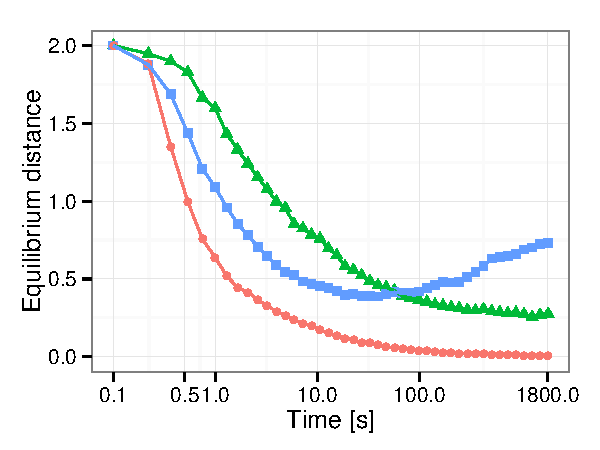
\includegraphics[width=\textwidth]{fig/convergence-IIGS_1_6}
\end{minipage}}
\subfigure[Aggregated]{\label{fig:GS-agg}
\begin{minipage}{0.24\textwidth}
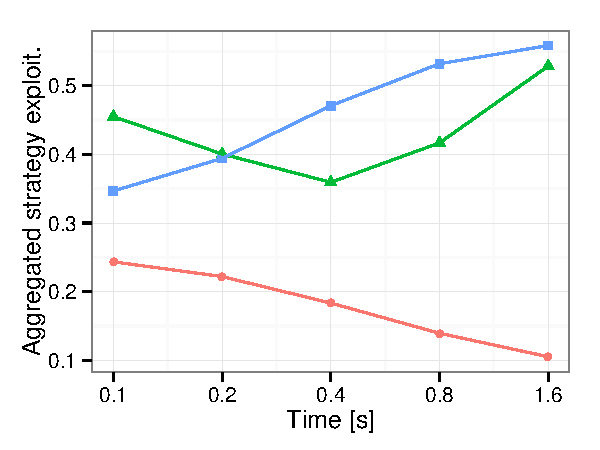
\includegraphics[width=\textwidth]{fig/agg_convergence-IIGS_1_6}
\end{minipage}}
\subfigure[OOS Params.]{\label{fig:GS-oos}
\begin{minipage}{0.24\textwidth}
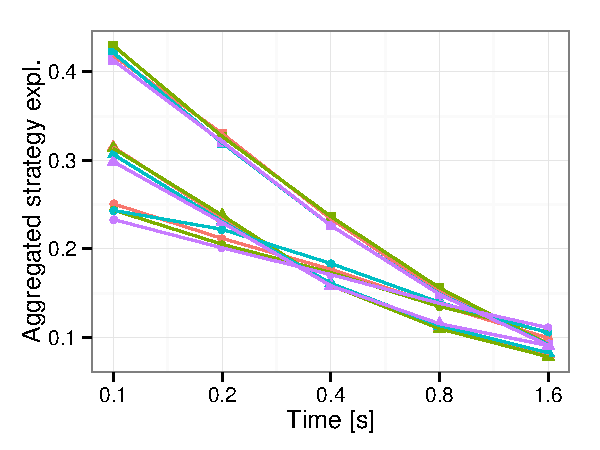
\includegraphics[width=\textwidth]{fig/agg_OSS_convergence-IIGS_1_6}
\end{minipage}}
\subfigure[Matches $\pm$3]{\label{fig:GS-matches}
\begin{small}
\begin{tabular}{@{}|@{}r@{}|@{~}c@{~}c@{~}c@{~}c@{}|}\hline
0.1s&OOS&UCT&RM&RND\\\hline
OOS&\textbf{51.4}&57.7&61.0&81.5\\
UCT&\textbf{51.2}&62.9&62.7&84.0\\
RM&\textbf{52.3}&70.6&73.1&87.8\\
RND&\textbf{17.1}&15.7&10.3&49.7\\
\hline
\end{tabular}
\end{small}
}
\rotatebox{90}{\hskip-1.5cm Liar's Dice (6,1,1)}
\subfigure[Root]{\label{fig:LD-root}
\begin{minipage}{0.24\textwidth}
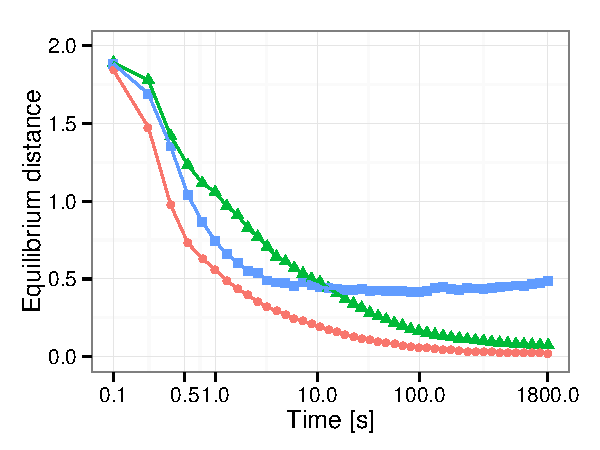
\includegraphics[width=\textwidth]{fig/convergence-LD_6_1_1}
\end{minipage}}
\subfigure[Aggregated]{\label{fig:LD-agg}
\begin{minipage}{0.24\textwidth}
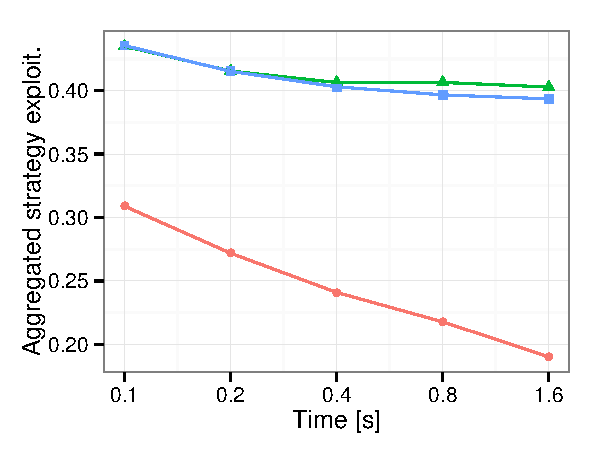
\includegraphics[width=\textwidth]{fig/agg_convergence-LD_6_1_1}
\end{minipage}}
\subfigure[OOS Params.]{\label{fig:LD-oos}
\begin{minipage}{0.24\textwidth}
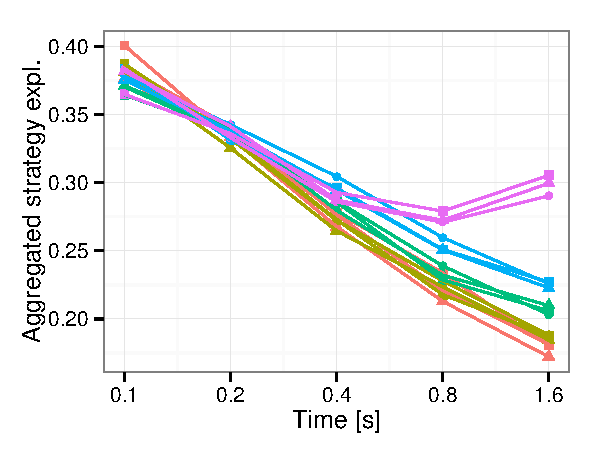
\includegraphics[width=\textwidth]{fig/agg_OSS_convergence-LD_6_1_1}
\end{minipage}}
\subfigure[Matches $\pm$4]{\label{fig:LD-matches}
\begin{small}
\begin{tabular}{@{}|@{}r@{}|@{}c@{~}c@{~}c@{~}c@{}|}\hline
0.1s&OOS&UCT&RM&RND\\\hline
OOS&\textbf{48.8}&\textbf{53.2}&\textbf{56.3}&\textbf{81.7}\\
UCT&41.3&50.0&50.8&82.3\\
RM&43.8&48.0&52.5&82.3\\
RND&17.8&19.2&17.5&47.5\\
\hline
\end{tabular}
\end{small}
}
\rotatebox{90}{\hskip-1.5cm Gen. Poker (2,2,3,3)}
\subfigure[Root]{\label{fig:GP-root}
\begin{minipage}{0.24\textwidth}
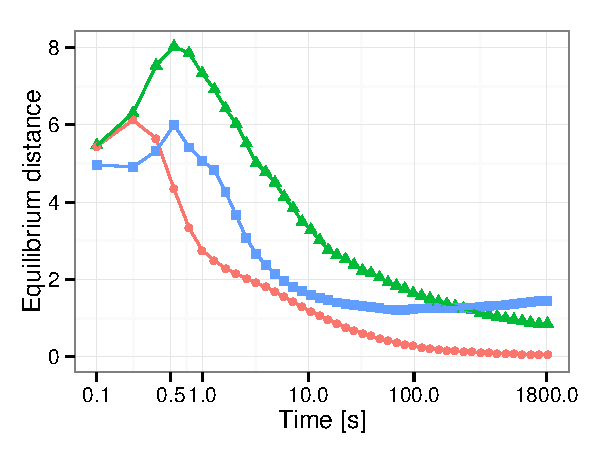
\includegraphics[width=\textwidth]{fig/convergence-GP_2_2_3_3}
\end{minipage}}
\subfigure[Aggregated]{\label{fig:GP-agg}
\begin{minipage}{0.24\textwidth}
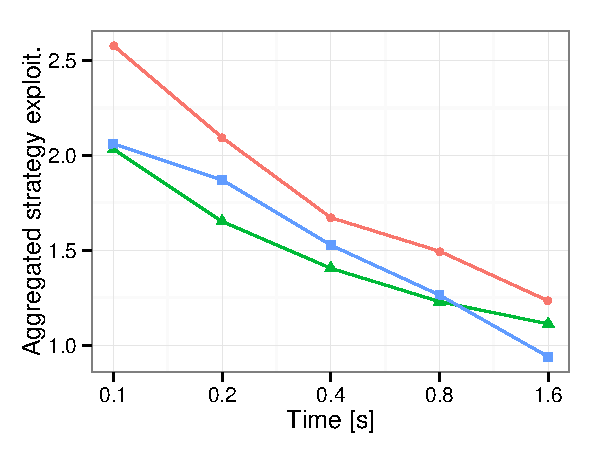
\includegraphics[width=\textwidth]{fig/agg_convergence-GP_2_2_3_3}
\end{minipage}}
\subfigure[OOS Params.]{\label{fig:GP-oos}
\begin{minipage}{0.24\textwidth}
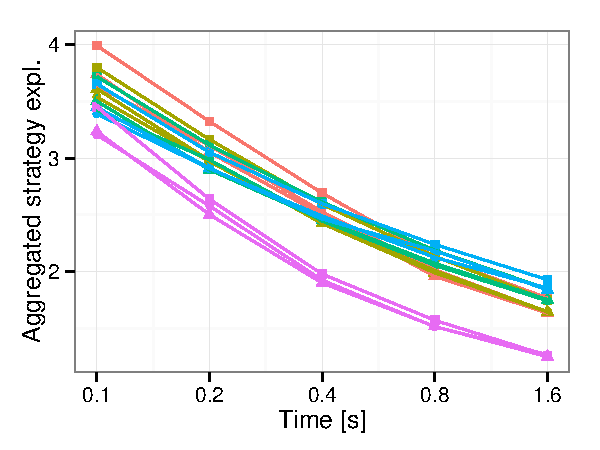
\includegraphics[width=\textwidth]{fig/agg_OSS_convergence-GP_2_2_3_3}
\end{minipage}}
\subfigure[Matches $\pm$0.84]{\label{fig:GP-matches}
\begin{small}
\begin{tabular}{@{}|@{}r@{}|@{\hspace{1pt}}c@{~}c@{~}c@{~}c@{}|}\hline
0.1s&OOS&UCT&RM&RND\\\hline
OOS&-0.37&-0.72&-0.43&2.63\\
UCT&0.25&0.10&-0.23&1.95\\
RM&0.50&0.17&-0.07&2.27\\
RND&-2.14&-1.62&-2.27&1.06\\
\hline
\end{tabular}
\end{small}
}
\caption{Exploitability and head-to-head performance in small variants of the evaluated games. The values after $\pm$ at the matches are the maximum size of the 95\% confidence intervals over all values in the table. (d) and (h) are win rates, while (l) is the difference of the  expected outcome of a pair of strategies and the value of the game.}\label{fig:small}
\end{figure*}


\begin{itemize}
\item running form the root, OOS clearly converges the fastest regardless of incremental tree building in all tree games
\item In aggregate exploitability, OOS produces less exploitable play than IS-MCTS with UCT and RM selection with the same amount of computation per move
\item In aggregate exploitability, OOS always perform better with more  time for any exploration and targeting < 1. For targeting =1, it breaks down as expected
\item In all tree games, with very short computation time (0.1s), higher targeting produces less exploitable strategies. With more time, less targeting yields better strategies, with the exception of targeting=1, which seems to be significantly better in GP. This indicates that non-locality does not cause problems in Poker.
\item head-to-head results in small games are mostly consistent with aggregated exploitability, OOS wins over IS-MCTS in II-GS and LD, while it looses in GP. In II-GS, OOS was the only algorithm that was not significantly loosing from the second position.
\item the performance form each position significantly differs for all algorithms, including OOS, which looses 
\item the amount of exploration in OOS has relatively small effect on exploitability in LD and GP, while it is significant in II-GS. It would be good to explain why.
\item the game playing performance in large game with limited time is bad. This is likely because the targeting costs a lot of computational resources and the untargeted portions of the tree are not visited/updated enough to fix the strategies anyway.
\end{itemize}



\begin{figure}
\centering

\subfigure[II Goofspiel (13)]{
\begin{small}
\begin{tabular}{@{}|@{}r@{}|@{~}c@{~}c@{~}c@{~}c@{}|}\hline
1s&OOS&UCT&RM&RND\\\hline
OOS&49.5(3.1)&25.4(2.7)&21.2(2.5)&72.8(2.7)\\
UCT&77.2(2.5)&70.0(2.8)&61.0(3.0)&90.6(1.8)\\
RM&79.8(2.4)&73.8(2.7)&67.5(2.9)&92.8(1.5)\\
RND&24.4(2.6)&6.2(1.5)&4.9(1.3)&49.0(3.0)\\
\hline
\end{tabular}
\end{small}
}

\subfigure[Liar's Dice (2,2)]{
\begin{small}
\begin{tabular}{@{}|@{}r@{}|@{~}c@{~}c@{~}c@{~}c@{}|}\hline
1s&OOS&UCT&RM&RND\\\hline
OOS&63.5(3.9)&33.7(3.8)&33.3(3.8)&86.2(2.8)\\
UCT&80.3(3.2)&48.2(4.0)&47.5(4.0)&85.8(2.8)\\
RM&80.3(3.2)&53.2(4.0)&52.7(4.0)&89.5(2.5)\\
RND&17.2(3.0)&15.3(2.9)&16.0(2.9)&49.3(4.0)\\
\hline
\end{tabular}
\end{small}
}

\subfigure[Generic Poker (4,6,4,4)]{
\begin{small}
\begin{tabular}{@{}|@{}r@{}|@{~}c@{~}c@{~}c@{~}c@{}|}\hline
1s&OOS&UCT&RM&RND\\\hline
OOS&-2.60(2.45)&-2.66(1.61)&-3.04(1.48)&9.94(2.33)\\
UCT&0.45(1.74)&-1.10(1.17)&-1.05(0.90)&8.02(1.89)\\
RM&0.90(1.76)&-1.35(1.24)&-0.32(0.92)&8.94(1.87)\\
RND&-5.61(2.08)&-4.44(1.40)&-4.67(1.35)&0.46(2.19)\\
\hline
\end{tabular}
\end{small}
}
\caption{Head-to-head matches in large variants of the games with 1s of computation per move and half of 95\% confidence intervals in the brackets.}
\end{figure}
